
\subsection{Demographic parameters}

The simulated values of adult female survival and post-senescent adult
female survival (Table \ref{tab:demo-pars}) resulted in effective
survival of 0.96, 0.95, 0.96 for stable, decreasing, and increasing
populations respectively. The expected CVs on adult female survival
were always lower when ICKMR was used than when IMR alone was applied
(mean decrease in CV = 0.02). The mean expected CVs were 0.02 (range
0.01-0.04), 0.01 (range 0.01-0.02), and 0.03 (0.01-0.06) for stable,
decreasing, and increasing populations respectively. Expected CVs
were less than 0.2 for all scenarios where CKMR was applied, but as
high as 0.06 when it was not. 

The simulated values of juvenile female survival were 0.9, 0.85, and
0.925 (Table \ref{tab:demo-pars}). Again, the expected CVs on juvenile
survival were always lower when ICKMR was used than when IMR alone
was applied (mean decrease in CV = 0.02). The mean expected CVs on
juvenile female survival were 0.06 (range 0.04-0.09), 0.03 (range
0.02-0.05), and 0.07 (range 0.05-0.07) for stable, decreasing, and
increasing populations respectively.

Across all demographic and sampling scenarios, the simulated proportion
of adult females in breeding state 2 was 0.26. The expected CVs varied
greatly depending on both demographic and sampling scenario, but were
notably lower when ICKMR was used compared to IMR (mean decrease in
CV = 0.82). The mean expected CVs on the proportion of adult females
in breeding state 2 were 0.54, 0.31, and 0.66 for stable, decreasing,
and increasing populations respectively.

See Appendix \ref{sec:Additional-results} Table \ref{tab:LH_Expected-CVs}
for expected CVs of life history parameters across all demographic
and sampling scenarios with and without the use of lethal samples
and ICKMR.

\subsection{Adult female abundance}

\begin{figure}
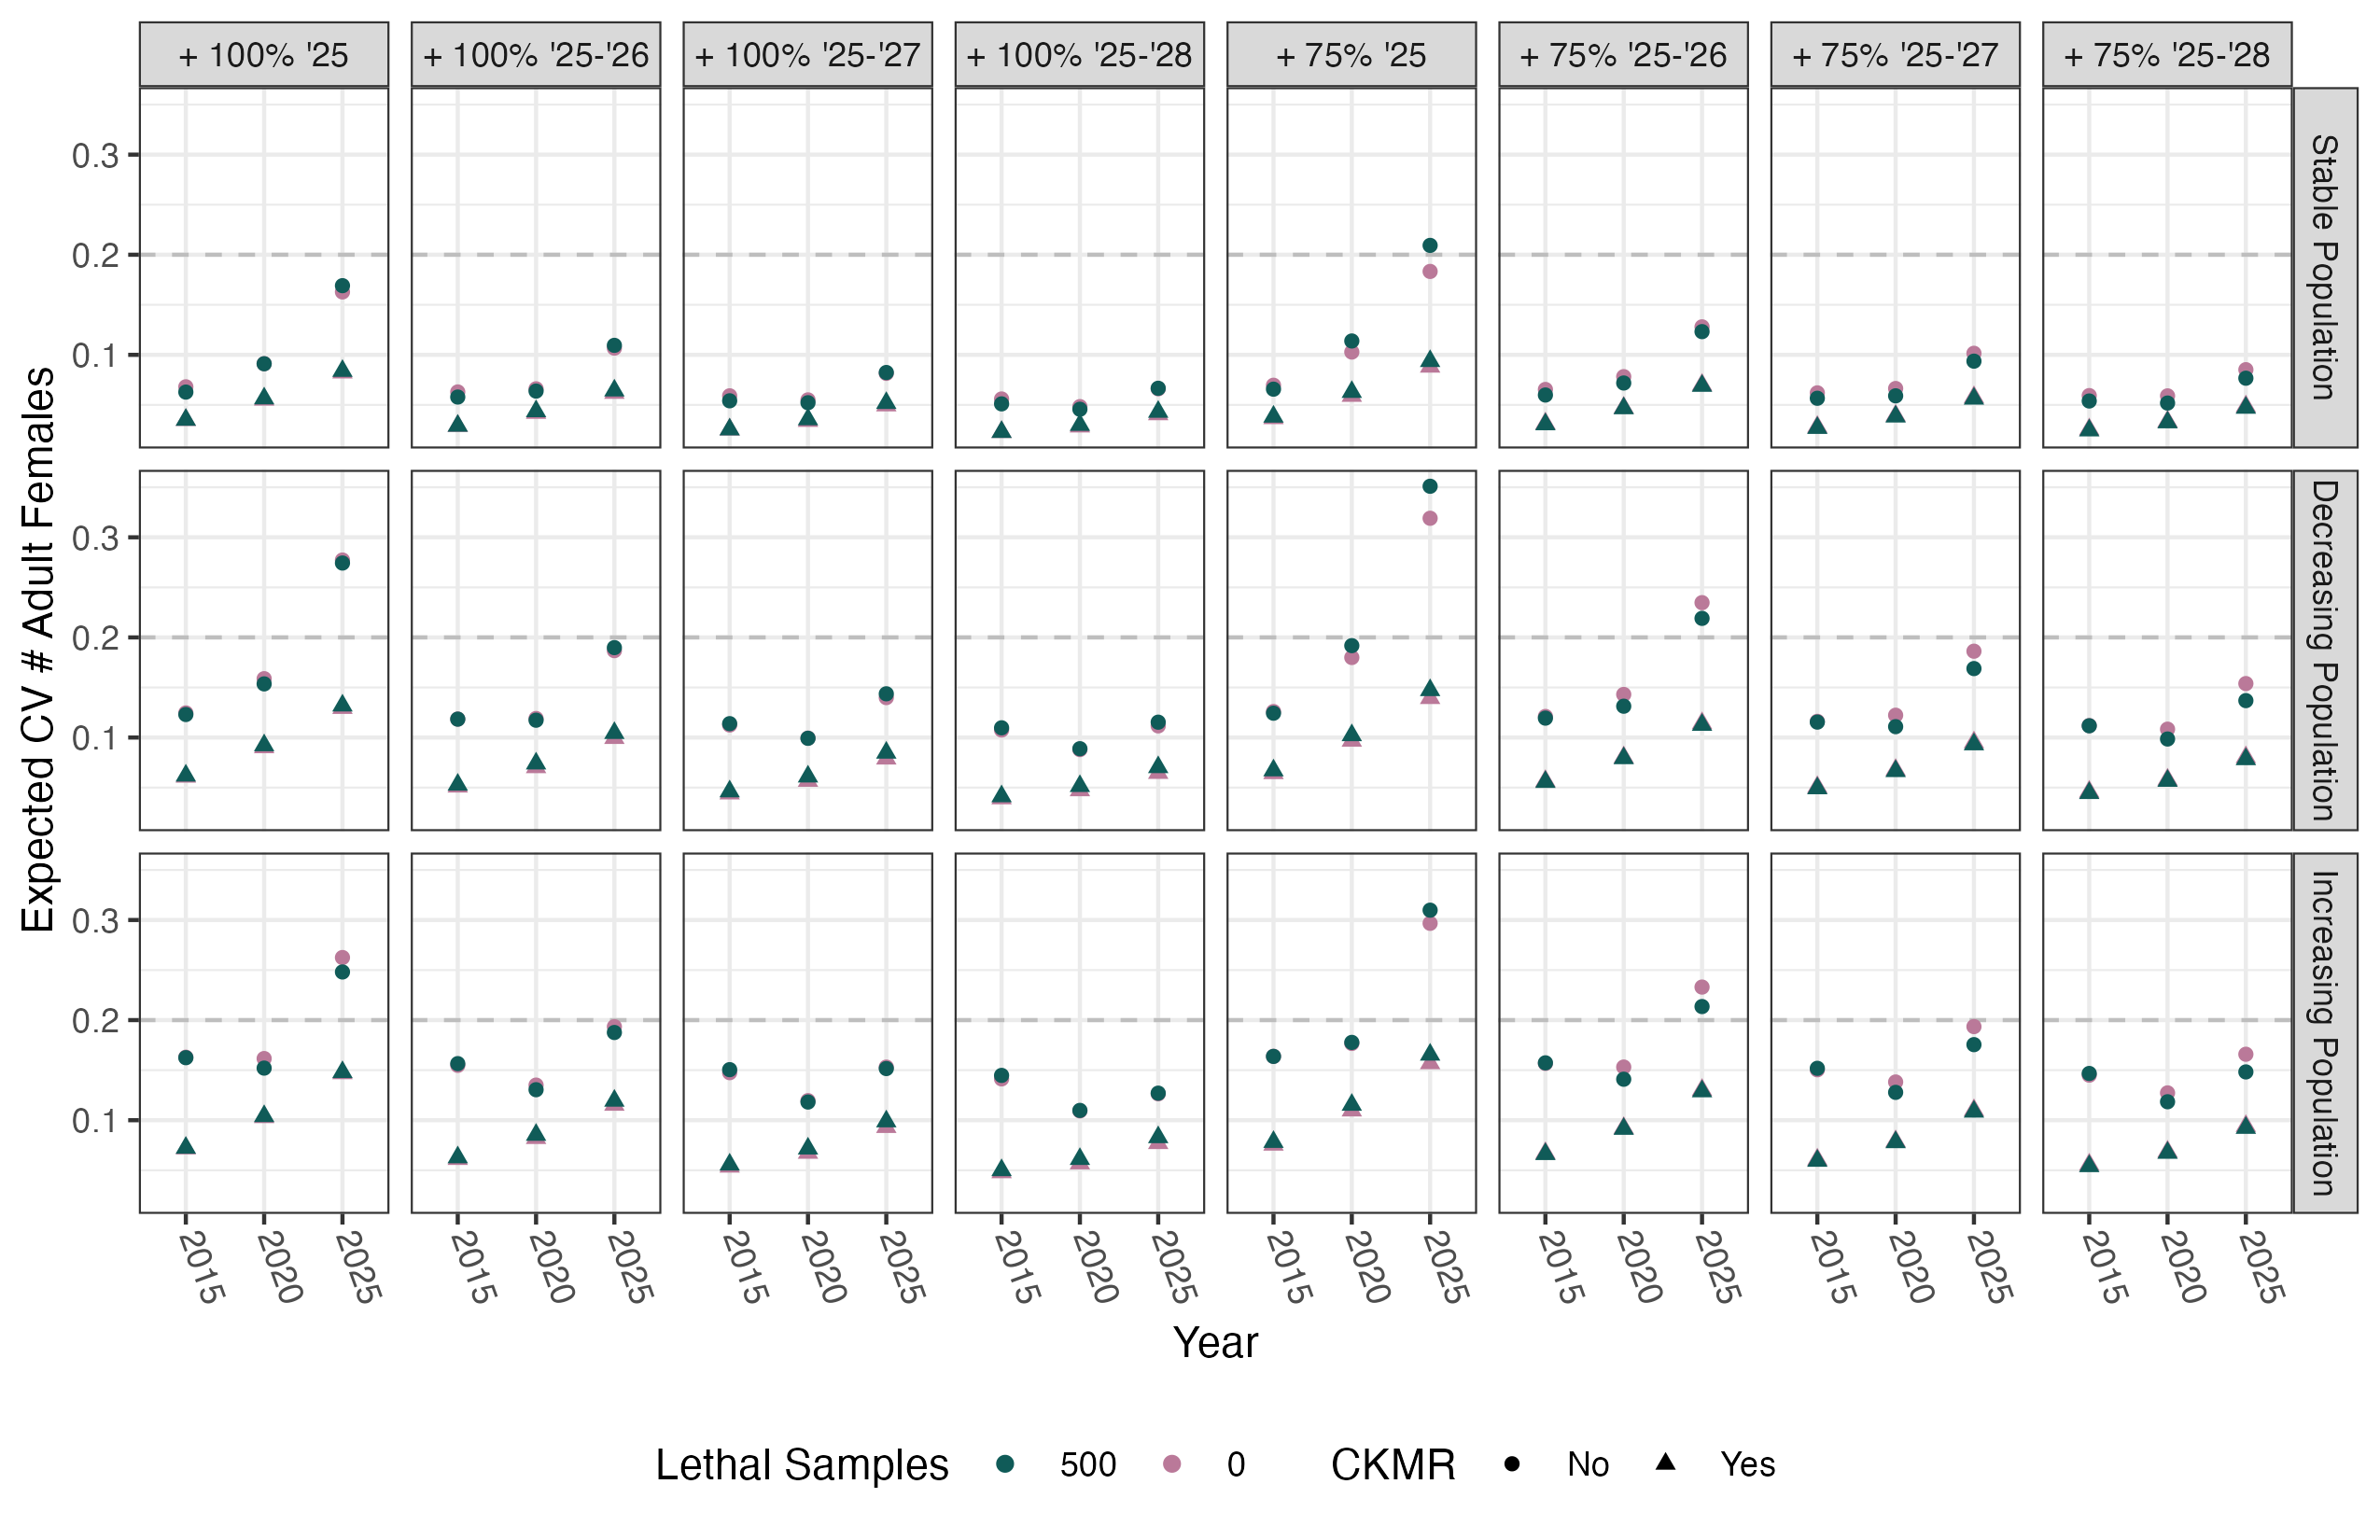
\includegraphics[scale=0.7]{../figures/MegaResults}

\caption{Expected CV of adult female abundance (vertical axis) in different
years (horizontal axis) under different demographic (panel rows) and
sampling (panel column) scenarios. Triangular points represent expected
CVs from IMR alone, while circular points show expected CVs with ICKMR.
The inclusion of lethal samples is indicated by green (lethal samples
included) or purple (no lethal samples included in sampling years)
points. The horizontal dashed line at CV = 0.2 represents an arbitrary
threshold for decision making.\label{fig:megaCV}}
\end{figure}

\begin{figure}
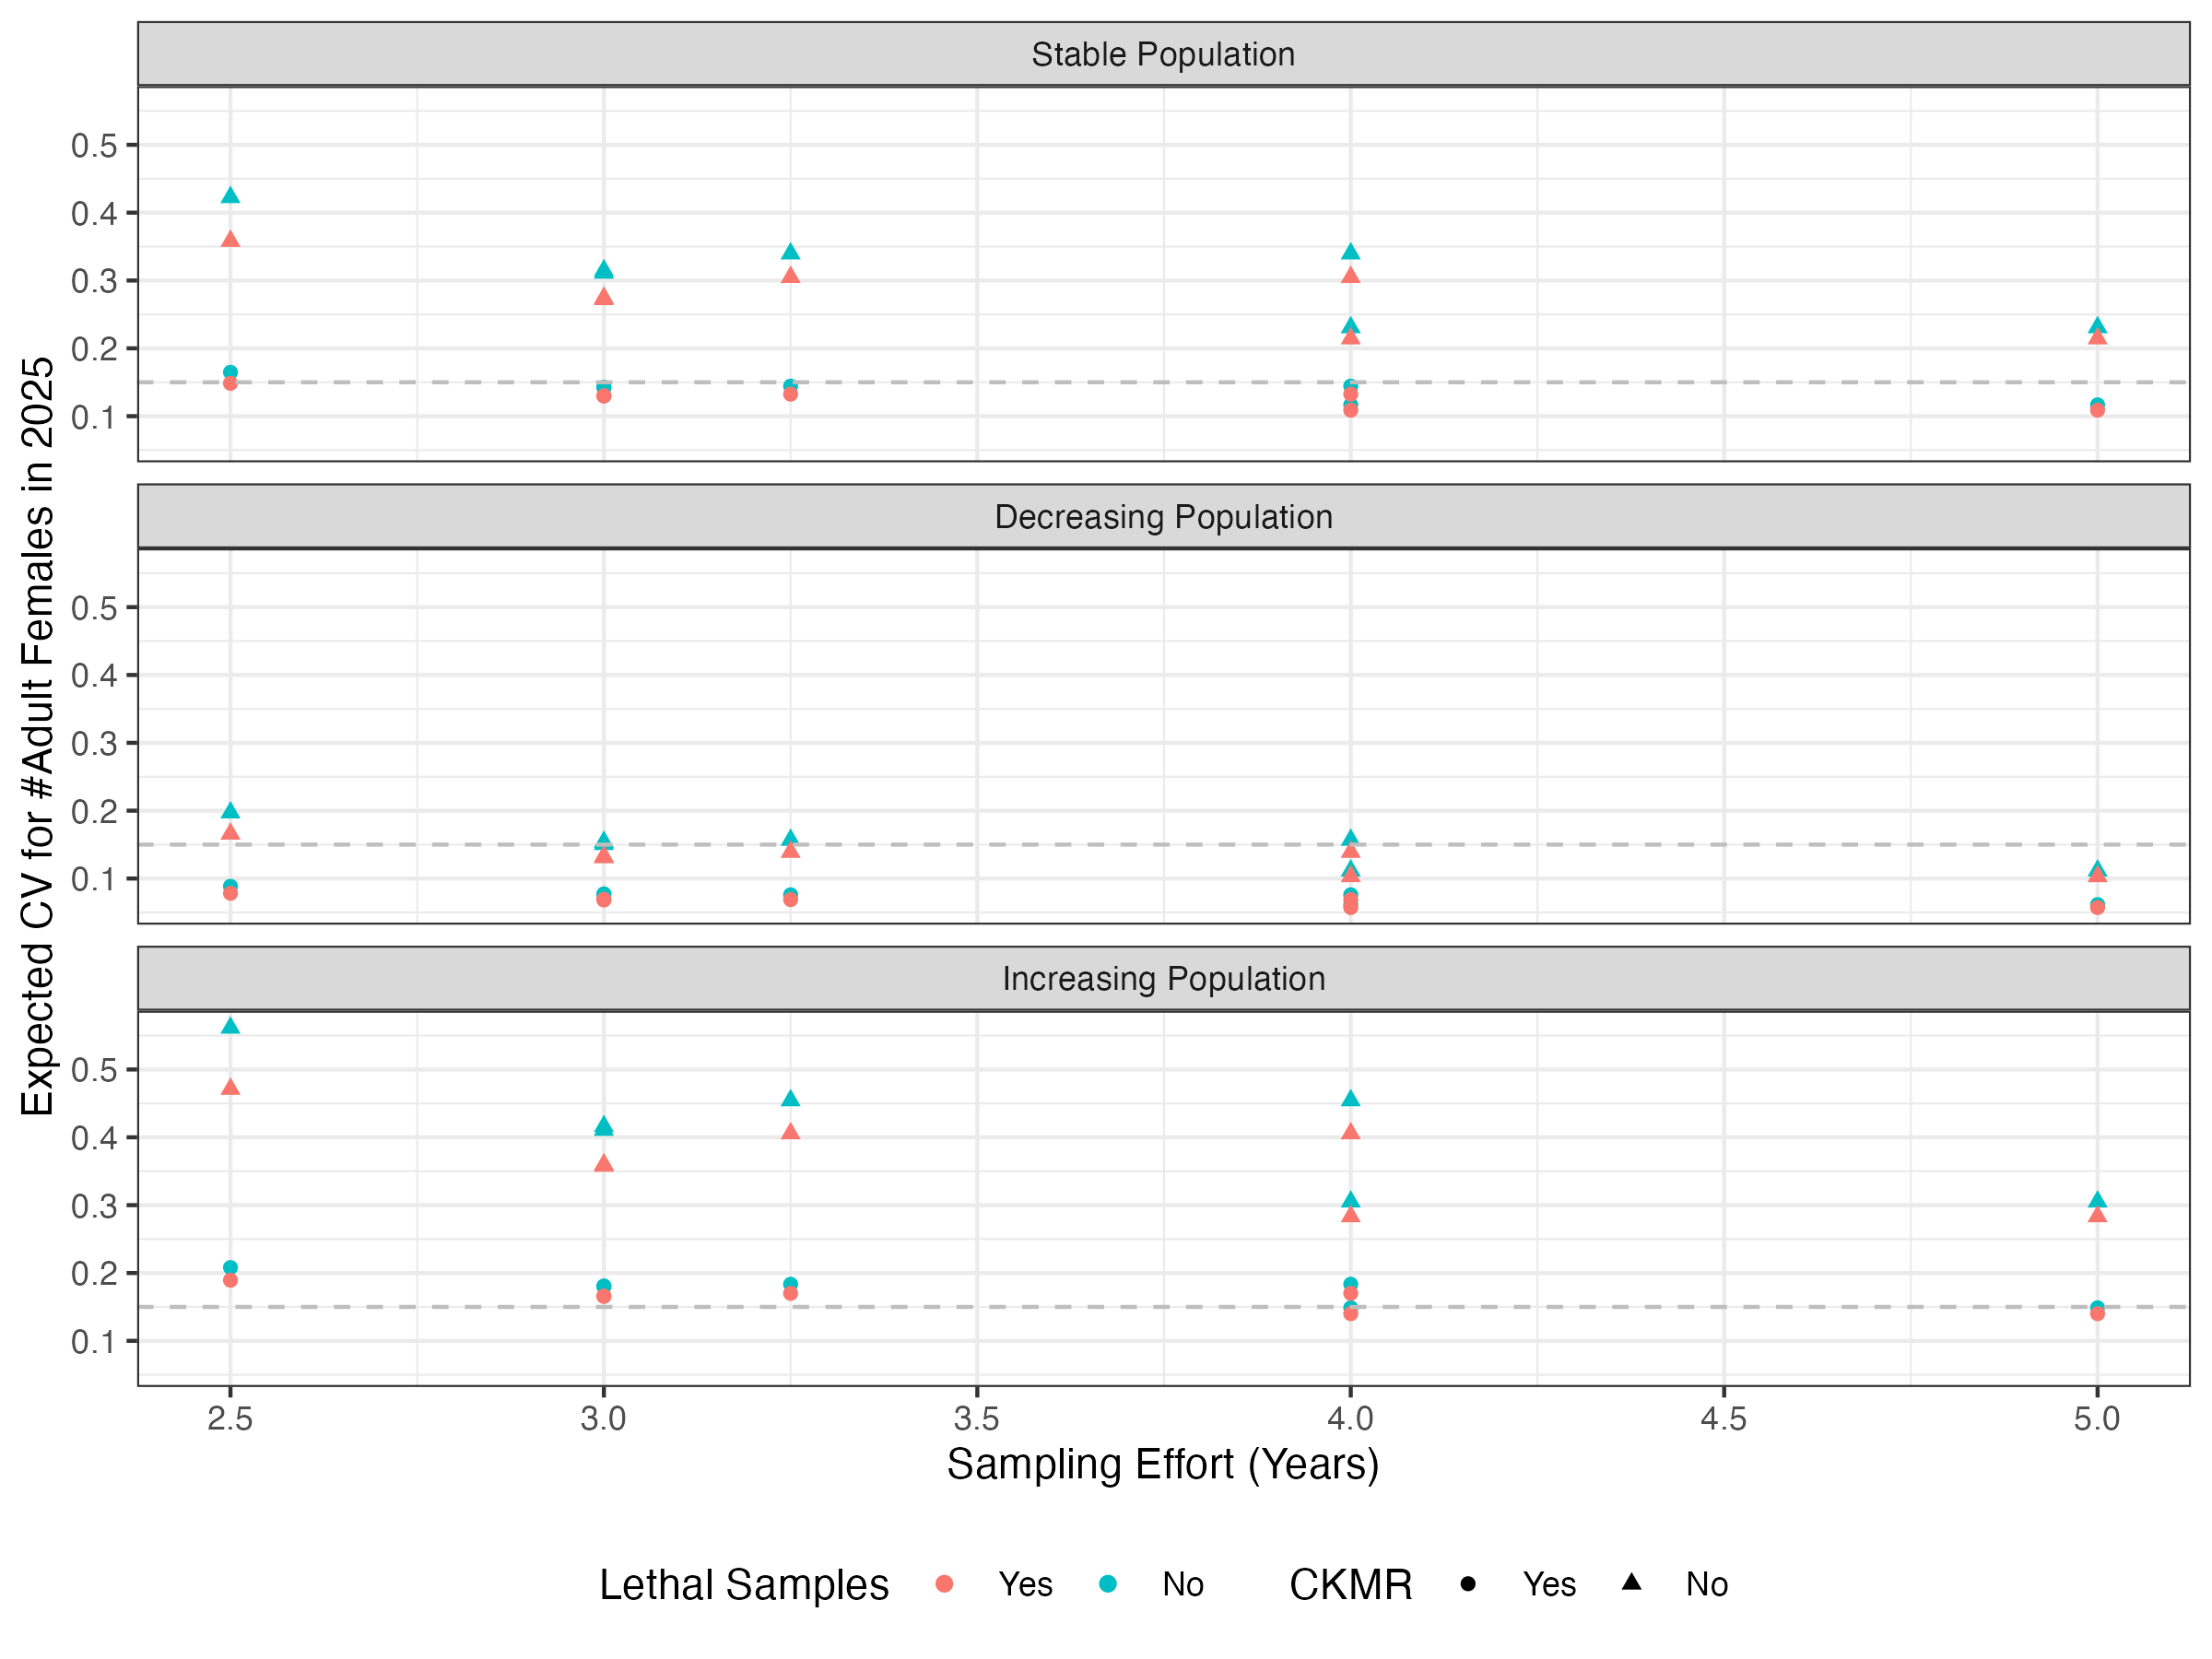
\includegraphics{../figures/EffortVCV}

\caption{Sampling effort (in number of years, horizontal axis) versus expected
CV for adult female abundance in 2025 with IMR alone (triangular points)
or with ICKMR (round points) and with (green points) and without (purple
points) the inclusion of lethal samples in sampling years. The three
panels represent demographic scenarios of a stable population, decreasing
population, and increasing population, respectively. The horizontal
dashed line at CV = 0.2 represents an arbitrary threshold for decision
making.\label{fig:effVcv}}
\end{figure}

\begin{figure}
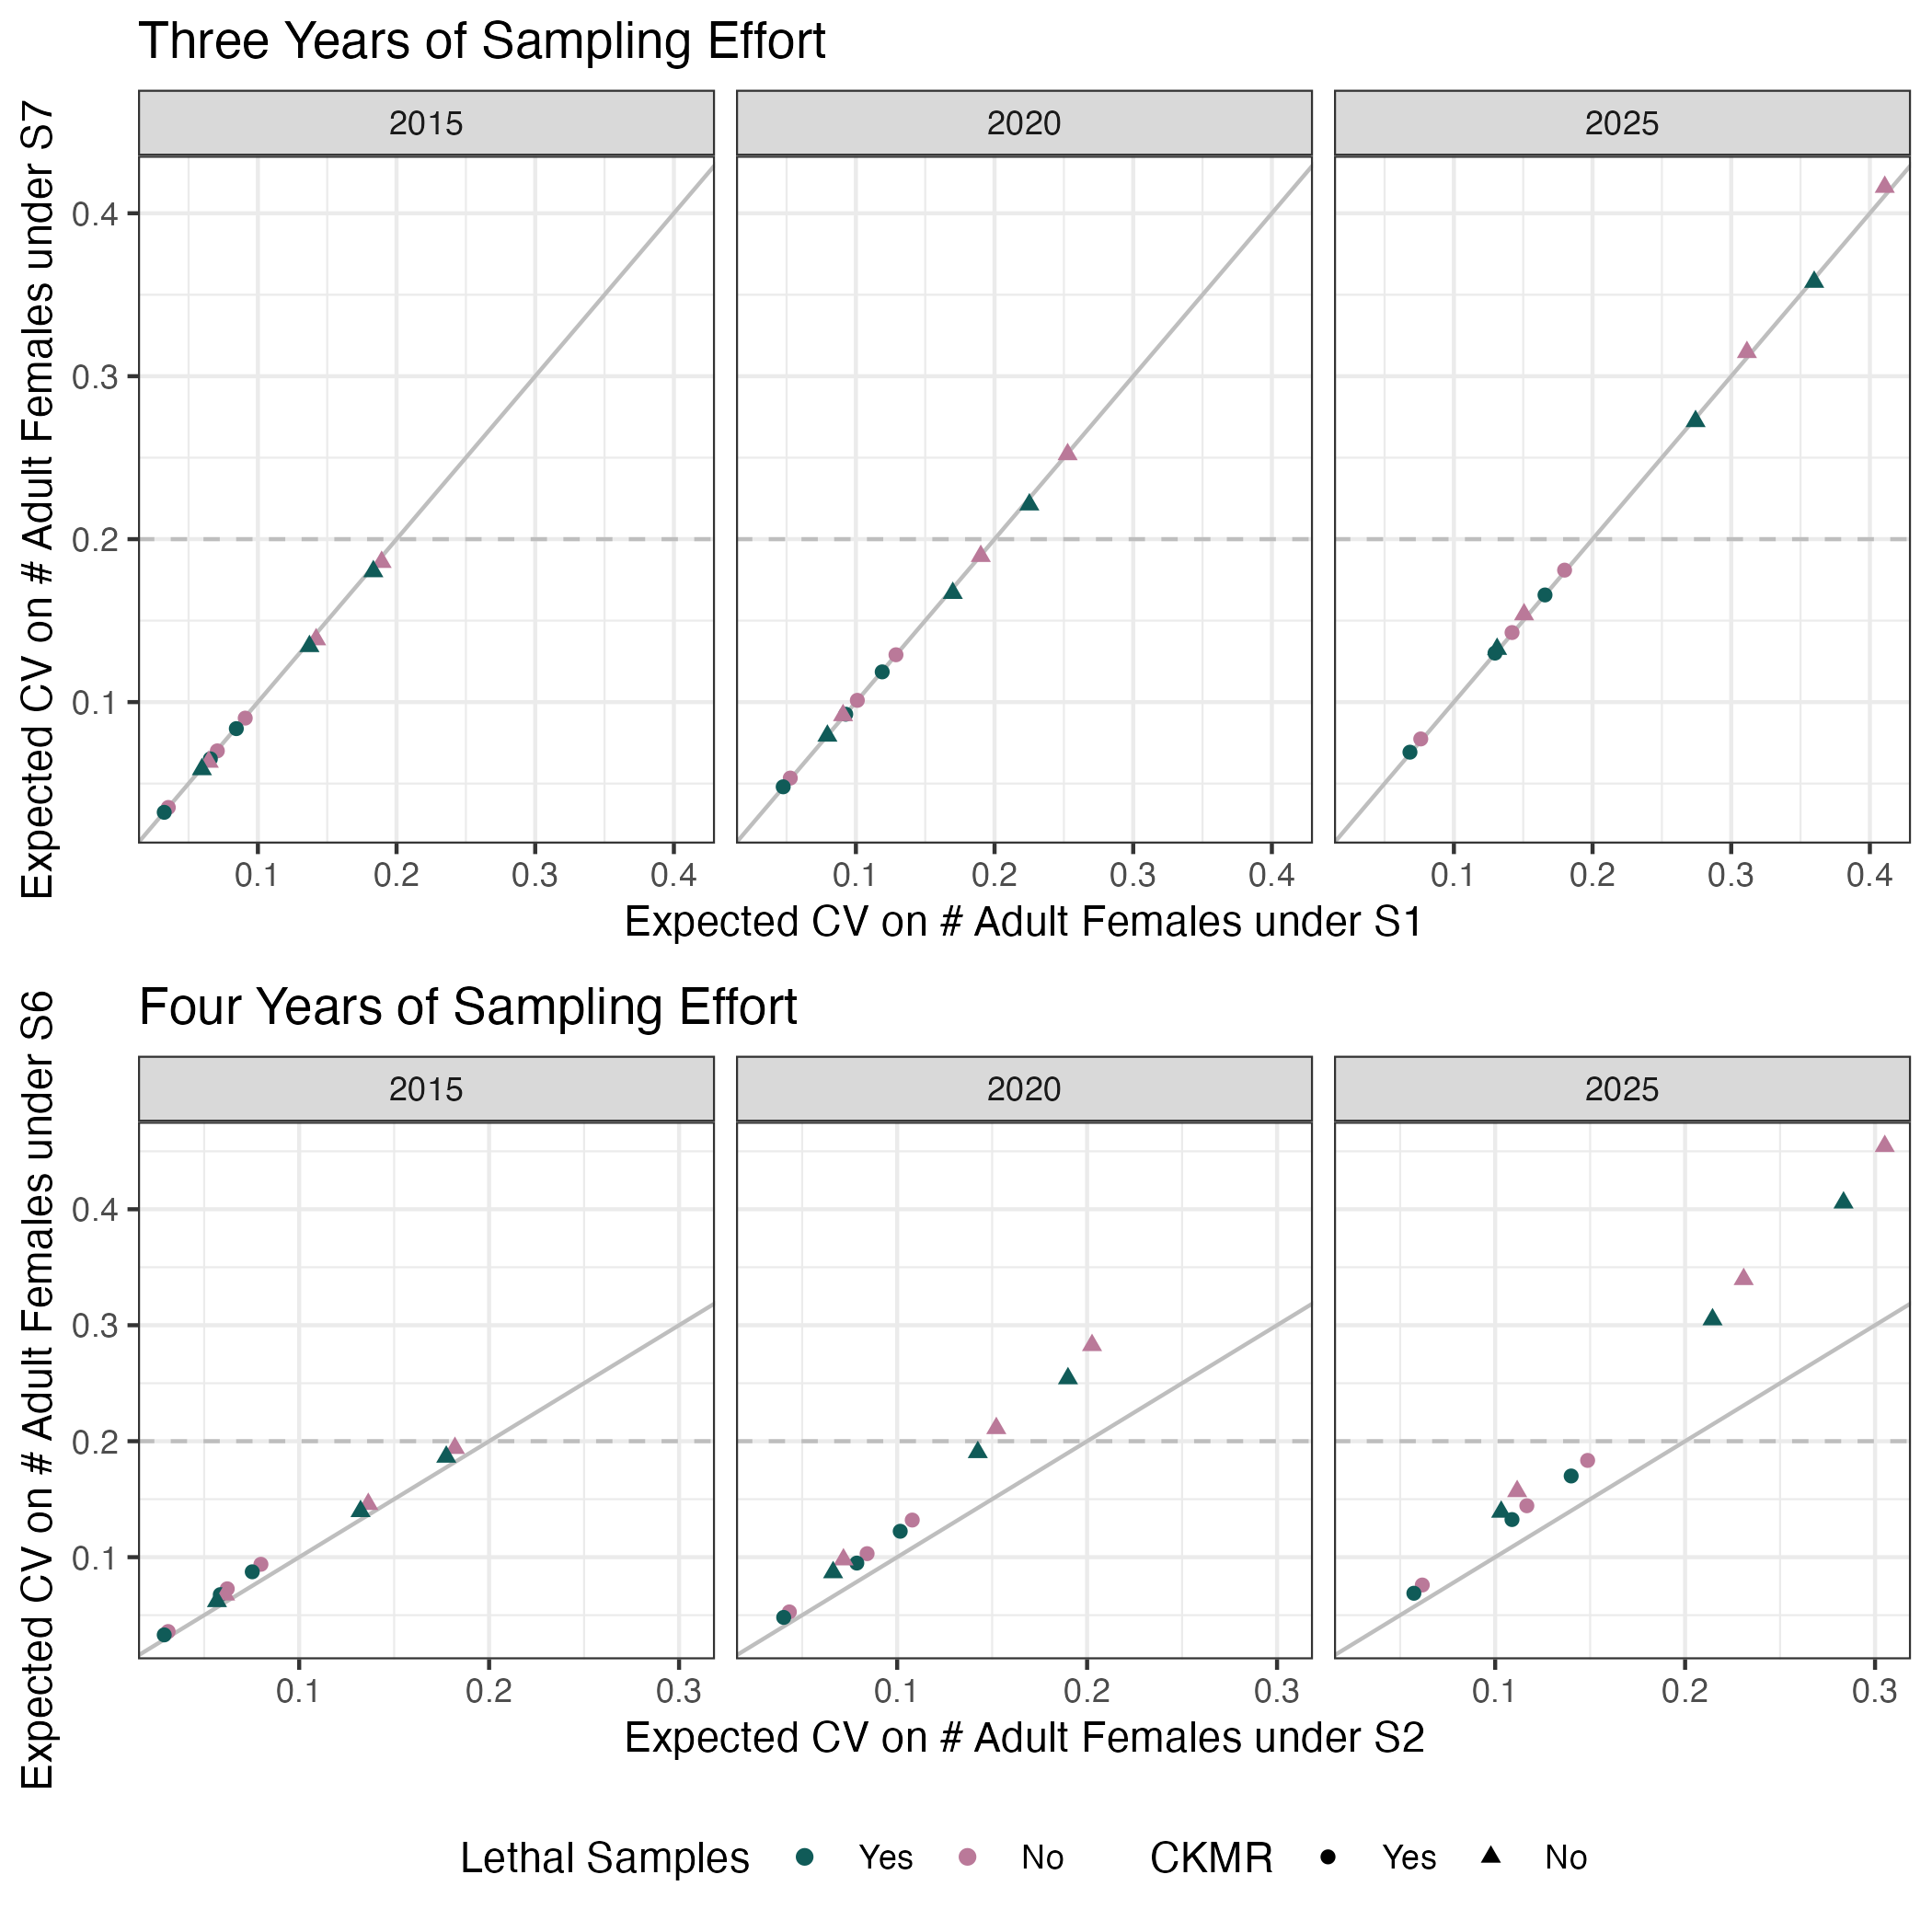
\includegraphics[scale=0.9]{../figures/CVsSameEffort}

\caption{Expected CV on the number of adult females with three years of sampling
(top panels) and four years of sampling (bottom panel). In the top
panel, the horizontal axis shows expected CVs under sampling scenario
1 and the vertical axis shows expected CVs under sampling scenario
7. In the bottom panels, the horizontal axis shows expected CVs under
sampling scenario 2 and the vertical axis shows expected CVs under
sampling scenario 7. From left to right, panels indicate expected
CVs in 2015, 2020, and 2025. Individual points represent expected
CVs under different possible demographic scenarios, with (green) and
without (purple) the inclusion of lethal samples, and with (round
points) and without (triangular points) the use of CKMR (versus IMR
alone). The solid grey line is 1:1. The horizontal dashed grey line
represents an arbitrary threshold CV of 0.2.\label{fig:cvWsameeff}}
\end{figure}

Across all demographic and sampling scenarios, the application of
ICKMR resulted in lower expected precision in estimates of abundance
compared to the application of IMR alone (Fig. \ref{fig:megaCV}).
The mean gain in CV on adult female abundance in paired scenarios
with and without ICKMR was 11\% for a stable population, 5\% for a
decreasing population, and 15\% for an increasing population. See
Appendix \ref{sec:Additional-results} Table \ref{tab:N_Expected-CV}
for expected CVs of adult female abundance across all demographic
and sampling scenarios with and without the use of ICKMR.

The demographic scenarios (see Table \ref{tab:demo-pars}) affected
expected precision of simulated survey designs in that a decreasing
population resulted in a smaller population size in the years of desired
inference (2015-2025) and therefore the number of kin pairs was higher
(and expected precision was lower) given a set number of samples (Fig.
\ref{fig:megaCV}, second row). Conversely, with an increasing population
size, the number of kin pairs resulting from a set number of samples
was lower, and therefore expected precision was higher (Fig. \ref{fig:megaCV},
third row). With an arbitrary target CV of 0.2 on estimates of adult
female abundance in 2015, 2020, and 2025, all demographic and sampling
scenarios resulted in sufficient precision when the population was
decreasing, while scenarios including ICKMR would be required to achieve
sufficient precision when the population was stable or increasing. 

Lethal samples provided greater gains in precision on abundance estimates
when only IMR was used; the mean gain in precision was 2\% when only
IMR was used but 1\% when ICKMR was applied. Note that when lethal
samples were included, we simulated the collection of 100 lethal samples
per year. We would expect the gain in precision for both IMR and ICKMR
to increase with an increased number of lethal samples. 

The simulated sampling scenarios resulted in between 2.5 and 5 years
of survey effort, where 5 years of survey effort was the original
plan for IMR (Fig. \ref{fig:effVcv}). When the population was simulated
to be stable or decreasing, sufficient precision in abundance estimates
could be achieved with as few as 2.5 years of survey effort when ICKMR
was applied and lethal samples were used. In scenarios when the population
was increasing, at least 3 years of survey effort would be required
even with the application of ICKMR and use of lethal samples. IMR
alone is expected to achieve sufficient precision only if the population
were decreasing. 

Some scenarios resulted in the same total number of years of sampling
but in different configurations (i.e., some had more calendar years
with less effort each year whereas others had fewer calendar years
with more effort each year). Scenarios 1 and 7 both resulted in 3
years of survey effort, while sampling scenarios 2 and 6 both resulted
in four years of sampling effort (Fig. \ref{fig:cvWsameeff}). Scenario
1 included sampling effort in 2023, 2025, and 2026, while scenario
7 included sampling in 2023, 2024, and 2025 (see Table \ref{tab:Sampling-scenarios}).
The expected CVs on estimates of adult female abundance in 2025, 2020,
and 2025 were comparable between these sampling scenarios (Fig. \ref{fig:cvWsameeff},
top panel). Scenario 2 included sampling in 2023, 2025, 2026, and
2027, while scenario 6 included sampling in 2023 and a lower level
of sampling (75\% effort) in 2025, 2026, 2027, and 2028. Expected
precision of abundance estimates was greater for scenario 6 than for
scenario 2 in all years of desired inference, with the greatest gains
in the 2025 estimate (Fig. \ref{fig:cvWsameeff}, bottom panel). This
suggests that more years of effort with fewer samples collected per
year could improve overall precision in estimates of adult female
abundance. {[}1178 words{]}.
